\documentclass{acm_proc_article-sp}
\usepackage{csquotes}
\usepackage{hyperref} % For hyperlinks in the PDF
\usepackage{url}
\usepackage{csquotes}
\usepackage{amsmath}
\usepackage{gensymb}
\usepackage{listings}
\usepackage{color}
\definecolor{lightgray}{rgb}{.9,.9,.9}
\definecolor{darkgray}{rgb}{.4,.4,.4}
\definecolor{purple}{rgb}{0.65, 0.12, 0.82}

\lstdefinelanguage{JavaScript}{
  keywords={typeof, new, true, false, catch, function, return, null, catch, switch, var, if, in, while, do, else, case, break},
  keywordstyle=\color{blue}\bfseries,
  ndkeywords={class, export, boolean, throw, implements, import, this},
  ndkeywordstyle=\color{darkgray}\bfseries,
  identifierstyle=\color{black},
  sensitive=false,
  comment=[l]{//},
  morecomment=[s]{/*}{*/},
  commentstyle=\color{purple}\ttfamily,
  stringstyle=\color{red}\ttfamily,
  morestring=[b]',
  morestring=[b]"
}

\lstset{
   language=JavaScript,
   backgroundcolor=\color{lightgray},
   extendedchars=true,
   basicstyle=\footnotesize\ttfamily,
   showstringspaces=false,
   showspaces=false,
   numbers=left,
   numberstyle=\footnotesize,
   numbersep=9pt,
   tabsize=2,
   breaklines=true,
   showtabs=false,
   captionpos=b
}

\begin{document}

\title{Pervasive computing: FSO Energy survey}
\subtitle{[Extended Abstract]}

\numberofauthors{2} %  in this sample file, there are a *total*
% of EIGHT authors. SIX appear on the 'first-page' (for formatting
% reasons) and the remaining two appear in the \additionalauthors section.
%
\author{
% You can go ahead and credit any number of authors here,
% e.g. one 'row of three' or two rows (consisting of one row of three
% and a second row of one, two or three).
%
% The command \alignauthor (no curly braces needed) should
% precede each author name, affiliation/snail-mail address and
% e-mail address. Additionally, tag each line of
% affiliation/address with \affaddr, and tag the
% e-mail address with \email.
%
% 1st. author
\alignauthor
Numa de Montmollin\\
       \affaddr{BeNeFri student}\\
       \email{numa.demontmollin@unifr.ch}
%% 2nd. author
\alignauthor
Thibaut Mauron\\
       \affaddr{BeNeFri student}\\
       \email{thibaut.mauron@unifr.ch}
}

\maketitle
\begin{abstract}

\end{abstract}

% A category with the (minimum) three required fields
\category{H.4}{Information Systems Applications}{Miscellaneous}
%A category including the fourth, optional field follows...
\category{D.2.8}{Software Engineering}{Metrics}[complexity measures, performance measures]

\terms{Practical project}

\keywords{Data representation, Web technologies, Graphs} % NOT required for Proceedings

\section{Introduction}
The Federal Statistic Office (FSO) building is an interesting example of what an actual smart building looks like. Build in 2000 it is designated to be energy efficient by using renewable energies and by monitoring many parameters. To save energy, they use much as possible renewable energy while providing a comfortable working place. Parameters that are monitored in real time, are shown in the following list:

\begin{itemize}
\item Interior temperature in each rooms
\item Outside temperature, sunlight and wind on each floors
\item Level of the different available energies
\item Consumption of the different used energies
\item State of the building like: knowing which windows are open or not or the position of each stores
\end{itemize}
 
From this list, we see that a lot of data are collected in a short period of time and raw data say nothing to the building manager. In consequence, we need a tool to represent the data in a readable and usable format.

Such a tool already exists and was created in the same time as the FSO building. Basically, it is composed of two parts: 

\begin{enumerate}
\item A software running on a specialized computer which receive live data, create report and draw graphs.
\item A computer which stores the data in plain text format without known backup
\end{enumerate}

The software produces a set of graphs and reports but it is impossible to do new graphs or configure it for new usage. For example, analysing the energy consumed compared to the outside temperature, the sunlight and the rain. It is possible for the building manager to monitor the existing sensor data, but not to take overall conclusions.Since the software runs on a specialized computer, it is really difficult to share or transmit graphs or reports in another manner than printing them!


The way, how the data is stored is an unusual story. At the beginning of the semester we had a meeting with  ???, one of the building manger to receive an extract of the stored data. But the evening before our meeting ??? did have a hearth attack (he went to the hospital and nfeels better now). In consequence, nobody else had access to the stored data because ??? was the only person to have granted access to the single computer holding that data.

Our goals for this project is to give anybody access to the data describing the building state, in regard to the energy consumption. As above, raw data is not sufficient to describe how energy the building consumes. In consequence, we need:

\begin{itemize}
\item To analyze the data and to represent it into graphs
\item Manage that every person with a screen terminal (Smartphone, personal computer, etc) and a Internet connection can visualize the data of the FSO building from everywhere
\item Define which kind of graph is representative for our use case, select the right data and comment it. Indeed, just generating dozen of graphs and make them available is not sufficient, since a not experimented user will be lost and unable to interpret them
\item The user must also be able to visualize data in the past in a time interval he or she is interested in
\end{itemize}

The interest behind giving access to that data to everybody is, that every person who wants to build a tool for representing the data can do it. To fulfil such a goal, the data must be stored on a database, accessible from the Internet through queries. Since, we are dealing with a lot of data, basic statistical operations should be able to be performed on the database.

Finally, this project will not provide a complete solution, but demonstrate how we could handle such a case, which tools we used and how difficult the task was.

According to our goals, we can conclude that the existing tool is not appropriate with what we want to realize. In the chapter \ref{approach} we will discuss how the tools must be used and configured according to our goals. In the chapter \ref{discuss} we will briefly discuss what our generated graphs represent and how they can be interpreted. Finally, in the chapter \ref{conclusion}, we will have a critic look at our work and discuss future outlook (\ref{future_work}).

\subsection{Description of the building}
The FSO building is composed of two different buildings: A tower, 60 meters high and the main building, four stages high with a flat roof. On the main building, rain water is collected and stocked in a tank (T1). The tank T1 is alimenting the flush of all the toilets of the two buildings. When the level of the tank T1 is under 20\%, water is bought to fill the tank up to 20\%. On the roof of the main building, $1200 m^2$ of solar panels are placed to warm the water of another of $25000m^3$ tank (T2). The heat of T2 is used to heat the building, when T2 is providing not enough heat, a gas heater is used to maintain a comfortable temperature. The building has nice system of ventilation based on the principle of convection, the high of the tower and a second wall over the windows. We do not explain it more, because we do not will treat the ventilation in the following of the report.

A lot of parameters are monitored, collected and send to a specialized computer. The figure \ref{fig1} gives an overview. The boxes in green are the data collected and used in our project, in red are the data collected.

\begin{figure}
\label{fig1}
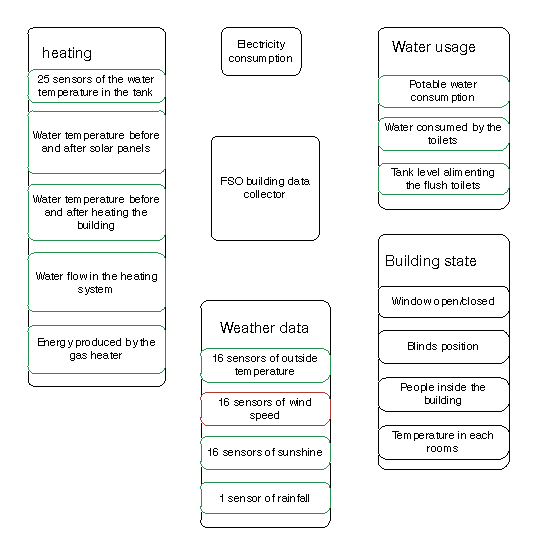
\epsfig{file=graph.eps}
\caption{Overview of data produced by the FSO building}
\end{figure}

\section{Approach}
\label{approach}
According to our goals of the previous section we decide to use Web technologies to create our tool and giving access to the stored data. Indeed, nowadays, every screen terminal, has access to Internet from almost everywhere and has a Web browser. With \texttt{HTML5}, \texttt{SVG}, \texttt{CSS3} and \texttt{Javascript} libraries it is now easy to create modern and responsive applications with a great user experience. Moreover, there exists plenty of \texttt{Javascript} and \texttt{SVG} libraries to generate graphs.

The choice of the database system is more difficult. From the course « Big Data » of Prof. Philipe Cudré-Maudoux we learned that a database system exists for almost every use cases. In our case, we want to be able to save a big amount of data who will grow among the time, to perform statistical queries and be easily accessible from every system. In consequence, we choose \texttt{ElasticSearch} (ES). Disadvantaged and advantages of ES are given in the section \ref{storing_data}.

\subsection{Simulation of the building}
In the section \ref{intro}, we see that ??? had a hearth attack and we cannot had access to the data. For this reason, we needed to simulate how the building is using and producing energy to have fake data.

Simulating exactly how the whole building is working is a complete work, which could be easily turn to a Master thesis. For this reason, our simulation is really basic, just some data are generated and is approximative, it does not reflect the reality. In our case, we generate data to build graphs. It means that the data must be coherent with them selves, with the input parameters and with the weather data. But they do not need to reflect the reality. It is important because for the suite of this project, graphs will be based on fake data and may be not representative.

Hopefully, we needed not to simulate all data. We found weather data on the Website Agroscope for the weather station of Cernier. From Agroscope \cite{agroscope}, we where able to collect from the 1st January 2007 to the 15th March 2015 with a period of one hour the following data:

\begin{itemize}
\item Rainfall in \(mm/h\)
\item Temperature in \(°C\)
\item Wind speed in \(km/h\)
\item Sunshine in \(W/m^2/h\)
\end{itemize}

From the weather data we simulated the following data wit a periodicity of one hour:

\begin{itemize}
\item Capacity of the water tank for the water usage of the toilets from the water usage and the rainfall. For the water usage, we defined a constant and we make it varying randomly but taking in account the hour of the day, the day of the week and if the day is a holiday or not.
\item Water bought to complete the capacity of the toilet water tank when not enough rainfall. The bought water is the water needed to fill the tank up to 20\% of is capacity when is capacity is under 20\%
 \item Temperature of the water heated by the sun in solar panel from the sunlight. It is the 60\% of energy of the sun to heat a certain amount of water at a certain temperature during one hour.
\item Temperature of the tank for the heating from the energy produced by the sun and the energy needed for heating.
\item Energy needed for heating from the exterior temperature and the heat latency
\item Energy from the gaz in complement of the sun energy for the heating
\item Interior temperature, varying of 0.5 \degree C in each 150 rooms
\item We also simulate that outside temperature was measured at 4 different high of the building at the 4 orientation (east, west, north, south).
\end{itemize}

What we can see from the list of the data we generated is that it is less complete that the data of the real building.

How we simulated the energy consumption is complicated:
\begin{enumerate}
\item Given the physic formula: $\Delta E = m*c* \Delta T$, where $\Delta E$ is the difference of energy in Joule, $m$ is the mass of the element, $c$ is the massic heat of the element and $\Delta T$ is the difference of temperature in \degree C. With the given formula, we calculate the increase of the temperature in the solar panel in one hour. For example, given 2000 Watts in one hour, the water temperature before the solar panel is at 60 \degree C and 100 liters are stocked in the solar panel. When we apply the formula we can calculate that the output water is at 85 \degree C.
$$85\degree C = 60 \degree C + \frac{2000W/h}{100l * 4.8\degree / kg}$$
\item The water heated by the panels is added to the tank water and we calculate the increasing of the temperature in the tank
\item We defined a linear function which determine how much energy is needed depending on the outside temperature to maintain a interior temperature of 21\degree C
\item We define a water debit in liter/hour send in the heating system. The debit is varying randomly
\item We define that the a certain amount of water at a temperature X at the input of the system will have the temperature of the interior temperature of the building at the output. This is incorrect, because it doesn’t take in account many parameters, for example the heat transfers. We did like this for simplicity
\item We calculate how much energy the tank water can give when sending a certain amount of water at a temperature X
\item The energy of the gaz heater is the difference between the energy the tank water can give the energy needed
\end{enumerate}

The way we proceed to simulate the energy is not accurate and in our simulation energy consumption will in fact depend of the sunshine, which is not true in the reality. We did not investigate any further because this solution is outputting coherent data with input data, it can be used to build graphs and our work is not simulate the building.
\subsection{Storing the data}
\label{storing_data}
ElasticSearch is a NoSQL database, designed to run a distributed system. The communication is done through a REST HTTP server \cite{Fielding2000} and data are exchanged through the Javascript Object Notation (JSON) \cite{json} format.

The advantages of choosing ElasticSearch are as follow:
\begin{itemize}
\item Designated to work on distributed systems, it means that the system can growth with ease with the quantity of saved data or if it needs to handle high traffic.
\item Complex statistical operation can be performed such as mean, minima, maxima, standard deviation, etc on a set of data. Data can as well be aggregated based on many parameters \cite{es_agg}. For example, we can query all the temperature of the last ten years wit one measure by hour, aggregate the data in a group of twenty-four hours and calculate, the mean, the standard deviation, minimum and maximum for each group of data and for the all data. All of that in one query with an easy syntax.
\item Preforming queries on the database is done through the HTTP protocol and query are written in JSON. For a developer, it is easy to handle HTTP request and he don’t need to learn another language for interacting with database. For example, we can imagine a case of an Web application which query elastic search directly from the browser without using a traditional Web server language.
\item An efficient index system who will index the most popular and complicated queries, increasing the response time
\end{itemize}
However, there exists disadvantages:
\begin{itemize}
\item When a query is malformed it is hard to debug it
\item Passing to a production environment is challenging
\item It is a young product and less stable than more older database systems
\end{itemize}

\subsection{Graphing the data}
As we said in chapter \ref{intro} our goal is to represent data about the energy management. Because we needed to simulate the data of the building, we have a limited amount of data. For this reason, we can only represent a limited number of basic graphs. Moreover, choosing the right statistical indicators to represent a system is a complete and dedicated work and is not a part of our work. For that we only choose three graphs to illustrate what could be done with more data and a person defining and choosing the right indicators.

The graphs we choose are as follows:
\begin{enumerate}
\item Represent how much energy is consumed for heating. We represent the outside temperature, the energy from the sun and the energy from the gaz. It should show us that when the temperature is cold, more energy is needed. The use of energy from the gaz should be more important when the temperature is cold and/or the sun is low.
\item Represent how much water is used and from which source. We represent the rainfall, the level of the water tank and the amount of water bought when not there is not enough water in the tank. We should see a diminution or an augmentation of the tank level, correlated to the rainfall. The amount of bought water should be correlated to the level of the tank 
\item Represent the cost of the energy of non renewable sources. This graphs is to summarize the two above graphs and to have a main unit. For this reason, we converted the energy cost in francs and we compared to weather data, the outside temperature and the rainfall in our case. We should see a augmentation of the cost when the temperature is cold and the rainfall is low.
\end{enumerate}

Because our data are on a period of 7 years with a granularity of one hour, the user needs to be able to select the period of time he want to visualize the data. To fulfill this goal, the user needs to be able to select the start date and the end data of the data through a calendar.

\subsubsection{Technologies used}
In the section \ref{approach}, we decided to use \texttt{Javascript}, \texttt{SVG} and \texttt{HTML5} to do a visual representation of the data. Given that point, we select a Javascript library, called \texttt{n3-lines-chart}\cite{n3}, which represent an array of data to a SVG graph. We choose this library for this simplicity of utilisation, the quality of the rendered graphs and the big amount of options available. To simplify the user interaction and to structure well our Javascript, we used a Javascript Framework called \texttt{AngularJS}\cite{angular}. Moreover, the library \texttt{n3-lines-chart} is designed to fit well with \texttt{AngularJS}. \texttt{AngularJS} is a Framework which aims to simplify both development and the testing of a Web application. It decouples the view rendering (user interface) to the application business logic with a Model View Controller architecture and by providing a small declarative language which can be used in the HTML pages.

Building a user interface in HTML/CSS/Javascript from scratch requires times and diverse competences in programming and design. To simplify our work, we used a HTML, CSS, Javascript Framework called Bootstrap. Bootstrap provides default styled elements (buttons, links, formular, etc), icons, typography and components. For example, Bootstrap provides navbar, dropdown and modal components.

For communicating with ES we used a small Javascript library, developed by \texttt{ElasticSearch} team \cite{es_javascript}, which simplify the communication and encode/decode \texttt{JSON} to Javascript objects. Though ES is accessible through \texttt{AJAX} requests, the \texttt{Javascript ElasticSearch} library simplify the development

We used as well two other utility library:
\begin{itemize}
\item \texttt{jQuery}\cite{jquery}, because it is required by Bootstrap and provides some useful functions
\item \texttt{moment}\cite{moment}, to manipulate the dates and times
\end{itemize}

For developing we used Brackets as code editor, \texttt{Bower} to manage Javascript and CSS libraries and \texttt{GruntJS} to simplify development task, such as:
\begin{itemize}
 \item Providing a basic \texttt{HTTP} server 
 \item Live reloading the browser when a HTML, CSS or JavaScript file is changed
\end{itemize}

\subsubsection{Low-pass Gaussian filter}
When we represent data, especially weather data, the user is not interested by the extrema of the data by the continuity and the change of the data. Typically, to know that at 6am the temperature is 2\degree C is not relevant but to see that the temperature is going down during the night, at 6am the temperature is at is lowest and is growing up during the day is more interesting. For that a low-pass Gaussian filter can be used to show a continuity over the data. The advantages of a low-pass Gaussian filter against a moving average is that data are closer to what they are with a better continuity [citation].

The principle of a Gaussian low-pass filter is simple. Given a central value, we take a k number of value at the left of the central value and a k number of value at the right of the central value. After that, we weight the all selected value following the rule:  As most a value is far from the central value as more is multiple value is low. Finally we addition all the value to have the new value of the central value.

For these reasons, we implemented a low-pass Gaussian filter for our project. We the help of the book[xxx], the implementation is easy and is done in a couple of minutes. But all the art is to choose the correct Gaussian scale. If we take a huge Gaussian scale, the curve will be flat and if we take a small Gaussian scale it will change nothing. In our project, the number of data change depending if the user choose to represent the data of one day or of one year. For that we implemented different Gaussian scale and we let the user choose is more appropriate scale. 

\subsubsection{Implementation}
For the implementation, the main work is to write the correct query to \texttt{ElasticSearch}. Indeed, the user interface is simple and Bootstrap do quite all the work. Drawing the graphs is done by the \texttt{n3-line-charts} library and interacting with the user is simplified a lot by \texttt{AngularJS}.

For writing the \texttt{ES} query, we need to take in account that a big amount of data could be returned. To avoid that, we need to group our data over a certain period of time and to do an average of the data in the period of time. We defined four period of time:
\begin{itemize}
\item One hour
\item Six hour
\item Twelve hour
\item One day
\end{itemize}

Depending of which period of time the user select, we try to choose the defined period of time which will output more or less 500 data. By experimentation, we defined that 500 hundred data was a optimal number of data to represent.

Finally, the listing\ref{es_request} show a typical request to ES at the URL:\\
\texttt{GET \url{http://localhost:9200/pervasive/data/_search?size=500}}

\lstinputlisting[language={JavaScript}, caption={A typical ElasticSearch request to gather data for our graphs}, label={es_request}]{es.js}

What we can see is that we define a first aggravation over a certain period of time and sub aggravation to do an average on the desired field for the defined period of time.

When this request is executed and the results returned, we loop through all data, transform it with our Gauss function and pass it to the library \emph{n3-lines-chart} which will render graphs.

Our system is designed to be as user friendly as possible. it means that when a user change a parameter (the start or end date or the Gaussian scale) a new request is issued to ES and results are updated immediately.

\section{Discussion of the data}
\label{discuss}
The first things we can say about our graphs is that they don’t represent the reality. For example, the figure XXX which represent the energy consumption for heating over the last year is not accurate. If we look carefully we see a pic of consumption in the month of June when the temperature are high. On the other hand, In the month of January - February, there is a less energy consumed as in June but the temperature are colder. We can explain that because the simulation is buggy and do not really simulate how the building is working.

For the two others graphs, the problem is the same. The goal of this work is not to simulate perfectly the building or to find the bests graphs to represent how the building is, but to show how it is possible to represent a big amount of data to a large public in a friendly way.

If we were building a real application with real data, we should think at what could change for the building manger, the FSO direction, the public the fact to observe in real time how the building is working and managed. Indeed, interacting graphs are a powerful tool to monitor a system and every person could compare the graphs to what it should be. For example, if the FSO direction say that the building is Minergie® and for the sustainable development and people can observe that the graphs show that not. It could cause trouble. In conclusion, we our really basics results, we can say that if we where building a real application, the power of public and interacting graphs should not be misestimate.

Say that our graphs are not accurate, but they are perfect to show what can be done when using the right tools.

Dire qu'il y a peu de graph, que d'en rajouter ne pose pas de problème, mais que cela n'apporte rien de plus au travail et qu'il nous manque des données.
\section{Conclusion}
\label{conclusion}
In the project, our goals was to implement a system for representing the data of the FSO building. More precisely to show how it possible to represent data with Web technologies and modern Big data systems.

For what we see it all along the section \ref{approach} we can say that doing data representation with Web and Big data technologies is a perfect working solution. Building graphs is an easy task when using the appropriate technologies and tools. In fact, building Web application do not requires big programming skills, but a good knowledge of which tools, libraries and technologies are existing and how to combine them.

In our project, the graphs we build was maybe not the most representative and they where based on fake data. Bur our project was not represent the best as possible how the FSO building is working but to show how we could do it. In this sense, our project fulfil his objectives because we give a nice way how to represent data through graphs with ease. Using Web and Big data technologies imply that distributing on almost platforms, for every type of user, having scalability and reliability is easy to setting up.

\subsection{Future work}
\label{future_work}
Here we will present some possible improvements of our project:

A first possibility would to add an interface in the application which is dedicated on building graphs. A user could choose which kind of data to combine in a graph, determine the graph (type, scale, axis, labels, etc) and apply statistical transformation on data (Gauss-filters, grouping, counting, etc). Such a tool already exists (Kibana), but is not enough configurable and adaptive for our case. The idea is to build a tool like Kibana but adapted to the representation of data of a Smart building. We could imagine that our tool could be used for every Smart building, or either groups of Smart building, and it only requires configuration to work across all the possible use case.

We could go more further and imagine that such tool could be used to managed a community of many houses where everybody can participate to the management of the energy depending of the needs and the available energy.

Another possibility would to extend the simulation part of our application and permit to simulate how a building is working and making prevision based on actual and paste data. Such a tool would be very useful for a building manager to try to optimize the energy consumption of the building. For example, what would change if I add $200m2$ of solar panel? Would the cost over investment be benefit? using such tool could help to save energy and to reduce the costs.



%ACKNOWLEDGMENTS are optional
\section{Acknowledgments}
We would like to thanks Mr ??? for his great help and the time he spends to explain to us and to do visiting the FSO building.

%
% The following two commands are all you need in the
% initial runs of your .tex file to
% produce the bibliography for the citations in your paper.
\bibliographystyle{abbrv}
\bibliography{sigproc}  % sigproc.bib is the name of the Bibliography in this case
\balancecolumns
% That's all folks!
\end{document}
